\documentclass[11pt,openany,oneside]{article}

\usepackage{makeidx}
\usepackage{latexsym}

\usepackage[latin1]{inputenc}
\usepackage[portuguese]{babel}
\usepackage[T1]{fontenc}
\usepackage{amsmath}
\usepackage{amsfonts}


%para criar o espacamento usual no primeiro paragrafo
\usepackage{indentfirst}

%package para fazer figuras a e b automaticamente
\usepackage{subfigure}
\usepackage[pdftex]{graphicx}

% para criar os links no texto quando cita equacoes, figuras, referencias, secoes, etc...
\usepackage{hyperref}

% para colorir os links criados anteriormente
\hypersetup{ colorlinks,
linkcolor=blue,
filecolor=darkgreen,
urlcolor=blue,
citecolor=blue }
\usepackage{graphicx,color}




\usepackage{amssymb}
\usepackage{amsthm}

% este define o espacamento entre as linhas
% para referencia, 1.5 'e um espacamento grande, utilizado na minha tese de doutorado
\renewcommand*{\baselinestretch}{1.2}

%comando para colocar vetor linha
%deve ser usado com o comando \vec{p}+\pvec{p}'=\pvec{p}''
\newcommand{\pvec}[1]{\vec{#1}\mkern2mu\vphantom{#1}}


%opcao 2 para acertar as margens
\usepackage{geometry}
 \geometry{
 a4paper,
 total={210mm,297mm},
 left=20mm,
 right=20mm,
 top=20mm,
 bottom=20mm,
 }  % o valor padrao das margens right, left, top e bottom e de 20 mm

% para incluir arquivos pdf, usando o comando \includepdf
\usepackage{pdfpages}

\pagenumbering{gobble} % remove o numero da pagina

%alinhar o texto
\usepackage[document]{ragged2e}


%macros para gerar o r cursivo do griffiths
\def\rcurs{{\mbox{$\resizebox{.09in}{.08in}{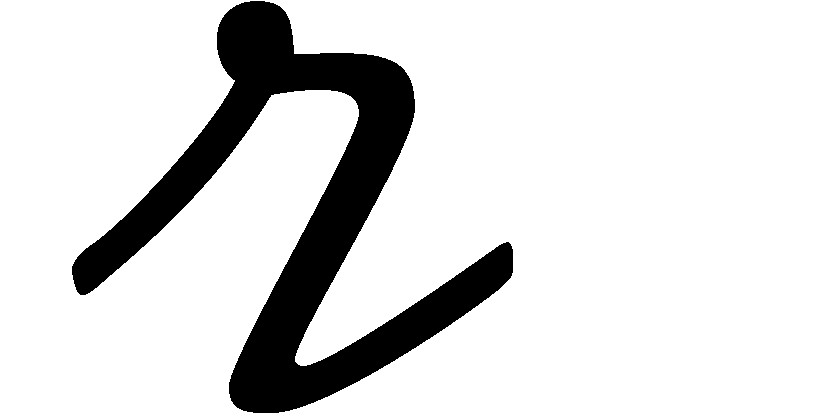
\includegraphics{ScriptR}}$}}}
\def\brcurs{{\mbox{$\resizebox{.09in}{.08in}{
\includegraphics{BoldR}}$}}}
\def\hrcurs{{\mbox{$\hat \brcurs$}}}


\begin{document}



\subsection*{Jata�, 03/02/16. Physics. UFG - Jata�.}

\subsection*{Exam 3. Eletromagnetism. Prof. Paulo Freitas Gomes.}

\vspace{0.2 in}
\noindent
Name: \noindent\rule{11cm}{0.5pt} 

\vspace{0.1 in}

\noindent
\textbf{1)} Suppose an electric and magnetic fields defined as
\begin{equation}
{\color{blue}\vec{E}(\vec{r},t) = - \dfrac{1}{4\pi \epsilon_0} \dfrac{q}{r^2} H(vt - r) \hat{r}, \qquad \vec{B}(\vec{r},t) = 0}
\end{equation}
where the Heaviside function is
\begin{equation}
{\color{blue}H (x) = \left\{
\begin{array}{rl}
 0 & \text{se  } x < 0  \\
\\
 1  & \text{se  } x > 0
\end{array} 
\right.} \nonumber
\end{equation}
\textbf{a)} Show that these fields satisfy the Maxwell equations. \textbf{b)} Calculate the charge $\rho$ and current $\vec{J}$ densities. \textbf{c)} Which physical situation can create such fields?


\vspace{0.1 in}
\noindent
\textbf{2) a)} A toroid has a rectangular cross section with a current $I$, $N$ tighly wound turns, inner radius $a$, outer radius $a+w$ and height $h$. Show that its magnetic field is:
\begin{equation}
{\color{blue}\vec{B} (\vec{r}) = \left\{
\begin{array}{rl}
 \dfrac{\mu_0 N I}{2\pi s} \hat{\phi} & \text{inside the toroid}  \\
\\
 0  & \text{outside the toroid  }
\end{array} 
\right.} \nonumber
\end{equation}
\textbf{b)} Now the current is increasing at a non-constant rate $dI/dt = kI$. If $w$ and $h$ are both much lower than $a$, find the electric field at a point $z$ above the center of the toroid.


\vspace{0.1 in}
\noindent
\textbf{3)} Suppose a magnetic monopole charge $q_m$ passes through a resistanceless loope of wire with self-inductance $L$. \textbf{a)} What current is induced in the loop? \textbf{b)} This is one of the methods used
to experimentally search for magnetic monopoles, see for example B. Cabrera, \textit{Phys. Rev. Lett.} \textbf{48}, 1378 (1982). From this Ref. would you say the magnetic monopole was observed? Why?


\vspace{0.1 in}
\noindent
\textbf{4)} There are many methods to solve differential equations (DE). One of them is to rewrite them in a simpler form. For example, the Maxwell equations are 4 first-order DE. \textbf{a)} Show that these equations can be written as these 2 second-order DE:
\begin{equation}
{\color{blue}\nabla^2 \vec{E} = \mu_0 \epsilon_0 \dfrac{\partial^2 \vec{E} }{\partial t^2}}, \qquad {\color{blue}\nabla^2 \vec{B} = \mu_0 \epsilon_0 \dfrac{\partial^2 \vec{B} }{\partial t^2}}
\end{equation}
\textbf{b)} What is the meaning of the fact that both $\vec{E}$ and $\vec{B}$ satisfy the wave equation?

\vspace{0.2 in}

\begin{flushright}
\begin{small}
\textit{ ... if you're willing to go through all the battling to get where you want to be, who's got the right to stop you? Maybe you got something you never finished, something you really want to do, something you never said to anyone, and you're told no, even after you paid your dues? Who's got the right to tell you no, who? Nobody! It's your right to listen to your gut, because you have the right to be where you want to be and do whatever you want to do!
}  
\textbf{Rocky Balboa}
\end{small}
\end{flushright}

 
\end{document}



